\documentclass[12pt,a4paper]{article}
\usepackage[a4paper, margin=0.8in, headheight=14pt]{geometry}
\usepackage{fontspec}
\usepackage{unicode-math}
\setmainfont{TeX Gyre Pagella}
\setmonofont[Scale=0.88]{TeX Gyre Cursor}
\setmathfont{Latin Modern Math}
\usepackage{xcolor}
\usepackage{colortbl}
\usepackage{titlesec}
\usepackage{enumitem}
\usepackage{tabularx}
\usepackage{booktabs}
\usepackage{array}
\usepackage{amsmath}
\usepackage{tikz}
\usetikzlibrary{shapes.geometric, arrows.meta, positioning, calc, fit, decorations.pathreplacing, decorations.pathmorphing, patterns}
\usepackage[american]{circuitikz}
\usepackage{tcolorbox}
\tcbuselibrary{skins, breakable}
\usepackage{hyperref}
\usepackage{fancyhdr}
\usepackage{graphicx}
\usepackage{microtype}
\hyphenpenalty=10000
\exhyphenpenalty=10000
\sloppy
\usepackage{caption}
\usepackage{setspace}
\usepackage{multirow}
\usepackage{tocloft}
\newcommand{\Q}[1]{\textbf{#1}\par\noindent\ignorespaces}
\definecolor{myred}{RGB}{196,30,58}
\definecolor{mydark}{RGB}{30,30,50}
\definecolor{mygreen}{RGB}{14,120,80}
\definecolor{myteal}{RGB}{0,130,140}
\definecolor{myamber}{RGB}{180,100,0}
\definecolor{mypurple}{RGB}{100,30,160}
\definecolor{mygray}{RGB}{246,247,249}
\definecolor{mgframe}{RGB}{180,185,200}
\definecolor{watermark}{RGB}{145,150,170}
\definecolor{hdrred}{RGB}{250,232,235}
\definecolor{hdrgreen}{RGB}{220,244,233}
\definecolor{hdrteal}{RGB}{220,242,244}
\definecolor{hdramber}{RGB}{253,242,215}
\definecolor{hdrpurple}{RGB}{238,228,255}
\definecolor{hdrgray}{RGB}{238,240,245}
\definecolor{rowalt}{RGB}{250,251,253}

\titleformat{\section}{\large\bfseries\color{myred}}{\thesection.}{0.5em}{}[\vspace{1pt}{\color{myred}\rule{\linewidth}{0.8pt}}]
\titleformat{\subsection}{\normalsize\bfseries\color{myteal}}{\thesubsection}{0.5em}{}
\titlespacing*{\section}{0pt}{18pt}{7pt}
\titlespacing*{\subsection}{0pt}{11pt}{4pt}
\setlength{\parindent}{0pt}
\setlength{\parskip}{4pt}
\renewcommand{\cfttoctitlefont}{\large\bfseries\color{myred}}
\renewcommand{\cftaftertoctitle}{\par\noindent{\color{myred}\rule{\linewidth}{0.8pt}}}
\setlength{\cftbeforetoctitleskip}{0pt}
\setlength{\cftaftertoctitleskip}{6pt}
\renewcommand{\cftsecfont}{\normalsize\bfseries\color{mydark}}
\renewcommand{\cftsecpagefont}{\normalsize\bfseries\color{mydark}}
\renewcommand{\cftsecleader}{\cftdotfill{\cftdotsep}}
\setlength{\cftbeforesecskip}{7pt}
\renewcommand{\cftsubsecfont}{\small\color{mydark}}
\renewcommand{\cftsubsecpagefont}{\small\color{mydark}}
\setlength{\cftbeforesubsecskip}{3pt}
\setlength{\cftsubsecindent}{1.4em}
\renewcommand{\cftpartfont}{\normalsize\bfseries\color{myteal}}
\renewcommand{\cftpartpagefont}{\normalsize\bfseries\color{myteal}}
\setlength{\cftbeforepartskip}{14pt}
\renewcommand{\arraystretch}{1.45}
\setlength{\tabcolsep}{6pt}
\arrayrulecolor{mydark}
\newcolumntype{B}[1]{>{\small\bfseries\raggedright\arraybackslash}m{#1}}
\newcolumntype{C}[1]{>{\centering\arraybackslash}m{#1}}
\newcolumntype{Y}{>{\small\raggedright\arraybackslash}X}
\renewcommand{\tabularxcolumn}[1]{m{#1}}
\newcommand{\currmodule}{Module 1}
\pagestyle{fancy}
\fancyhf{}
\fancyhead[L]{\small\color{myred}\textbf{HS-HU601}\;\color{mydark}--- Economics for Engineers}
\fancyhead[R]{\small\color{myteal}\textbf{\currmodule\ Notes}}
\fancyfoot[C]{\small\color{mydark}\thepage}
\fancyfoot[R]{\small\color{watermark}\textit{\copyright\ Biraj}}
\renewcommand{\headrulewidth}{0.5pt}
\renewcommand{\footrulewidth}{0.3pt}

\hypersetup{colorlinks=true, linkcolor=myteal, urlcolor=myteal,
  pdfauthor={Biraj Sarkar},
  pdftitle={HS-HU601 --- Combined Notes}}

\tcbset{
  tikzbox/.style={
    colback=mygray, colframe=mgframe, boxrule=0.6pt, arc=4pt,
    left=8pt, right=8pt, top=6pt, bottom=6pt,
    colbacktitle=mgframe, coltitle=mydark,
    fonttitle=\small\bfseries
  },
  defbox/.style={
    colback=hdrgreen, colframe=mygreen, boxrule=0.8pt, arc=4pt,
    left=9pt, right=9pt, top=6pt, bottom=6pt,
    colbacktitle=mygreen, coltitle=white,
    fonttitle=\small\bfseries
  },
  formulabox/.style={
    colback=hdrteal, colframe=myteal, boxrule=0.8pt, arc=4pt,
    left=9pt, right=9pt, top=7pt, bottom=7pt,
    colbacktitle=myteal, coltitle=white,
    fonttitle=\small\bfseries
  },
  examplebox/.style={
    colback=hdramber, colframe=myamber, boxrule=0.8pt, arc=4pt,
    left=9pt, right=9pt, top=6pt, bottom=6pt,
    colbacktitle=myamber, coltitle=white,
    fonttitle=\small\bfseries
  },
  masonbox/.style={
    colback=hdrpurple, colframe=mypurple, boxrule=0.8pt, arc=4pt,
    left=9pt, right=9pt, top=6pt, bottom=6pt,
    colbacktitle=mypurple, coltitle=white,
    fonttitle=\small\bfseries
  },
  exambox/.style={
    colback=hdrpurple, colframe=mypurple, boxrule=1pt, arc=5pt,
    left=10pt, right=10pt, top=8pt, bottom=8pt,
    colbacktitle=mypurple, coltitle=white,
    fonttitle=\bfseries,
    breakable, title after break={\textbf{Frequently Asked / Viva Questions (contd.)}}}
}
\tcbset{breakable}
\tcbset{after={\color{black}}}

\tikzset{
  block/.style={rectangle, draw=myteal, fill=hdrteal,
    text width=2.4cm, align=center, minimum height=0.95cm,
    font=\small, rounded corners=3pt, line width=0.7pt},
  redblock/.style={rectangle, draw=myred, fill=hdrred,
    text width=2.4cm, align=center, minimum height=0.95cm,
    font=\small, rounded corners=3pt, line width=0.7pt},
  netnode/.style={rectangle, draw=myteal, fill=hdrteal,
    text width=1.5cm, align=center, minimum height=0.8cm,
    font=\small, rounded corners=3pt, line width=0.7pt},
  sumjunc/.style={circle, draw=myamber, fill=hdramber,
    minimum size=0.62cm, font=\small, line width=0.8pt},
  snode/.style={circle, draw=mypurple, fill=hdrpurple,
    minimum size=0.55cm, font=\footnotesize, line width=0.7pt},
  arrow/.style={-Stealth, thick, color=mydark},
  redarrow/.style={-Stealth, thick, color=myred},
  line/.style={thick, color=mydark}
}

\newcommand{\modulestart}[2]{%
  \clearpage
  \renewcommand{\currmodule}{Module #1}%
  \renewcommand{\theHsection}{mod#1.\arabic{section}}%
  \renewcommand{\theHsubsection}{\theHsection.\arabic{subsection}}%
  \renewcommand{\theHsubsubsection}{\theHsubsection.\arabic{subsubsection}}%
  \phantomsection
  \addcontentsline{toc}{part}{Module #1: #2}%
  \setcounter{section}{0}%
  \begin{center}
    \vspace*{1.0cm}
    {\Huge\bfseries\color{myred} Module #1}\\[10pt]
    {\Large\bfseries\color{mydark} #2}\\[10pt]
    {\color{myred}\rule{0.55\linewidth}{1.2pt}}
  \end{center}
  \vspace{14pt}
}
\begin{document}

\thispagestyle{empty}

% ─── Page Border (TikZ Overlay) ────────────────────────────────────────────────
\begin{tikzpicture}[remember picture, overlay]
  % Outer border (fine line in mgframe)
  \draw[color=mgframe, line width=1.5pt] 
    ($(current page.north west) + (0.6in, -0.6in)$) rectangle 
    ($(current page.south east) + (-0.6in, 0.6in)$);
  % Inner border (finer accent line in myred)
  \draw[color=myred, line width=0.8pt] 
    ($(current page.north west) + (0.65in, -0.65in)$) rectangle 
    ($(current page.south east) + (-0.65in, 0.65in)$);
\end{tikzpicture}

\vspace*{1.0cm}
\begin{center}
  {\Huge\bfseries\color{myred} HS-HU601}\\[10pt]
  {\LARGE\bfseries\color{mydark} Economics for Engineers}\\[20pt]
  {\color{myred}\rule{0.7\linewidth}{1.5pt}}\\[18pt]
  {\Large\color{myteal}\textbf{Combined Module Notes}}\\[8pt]
  {\large\color{mydark} Modules 1 -- 4}\\[40pt]
  {\normalsize\color{mydark} Semester VI \quad$\bullet$\quad ECE \quad$\bullet$\quad 3 Credits}\\[12pt]
  {\normalsize\color{mydark} CGEC \;$|$\; B.Tech ECE (2023--27)}
\end{center}
\vspace{1.0cm}
\begin{center}
  \begin{tcolorbox}[colback=mygray, colframe=mgframe, boxrule=0.5pt, arc=3pt, width=0.85\linewidth]
    \centering\small\color{mydark}
    \textbf{Disclaimer / Study Guide Notice:}\\
    These are condensed \textbf{Short Notes} focusing on core theory, key formulas, block/circuit diagrams, and standard viva Q\&As for university exam revision. Exhaustive numerical practice problems and derivation edge cases are not covered. This serves as a quick-revision reference guide for students.
  \end{tcolorbox}
\end{center}
\vfill
\vspace{0.6cm}
\begin{center}
  {\large\bfseries\color{mypurple} Biraj Sarkar}\\[16pt]
  {\footnotesize\color{watermark}\textbf{IN ASSOCIATION WITH}}\\[8pt]
  {\small\bfseries\color{mydark} MAKAUT Wingman \quad$\bullet$\quad MAKAUT Future Minds}\\[12pt]
  {\large\bfseries\color{myteal} Cooch Behar Government Engineering College}
\end{center}
\vfill
\begin{center}{\small\color{watermark}\textit{Exam-Ready Notes}}\end{center}
\clearpage

\hypersetup{linkcolor=mydark}
\tableofcontents
\hypersetup{linkcolor=myteal}
\clearpage

% -- Module 1 -----------------------------------------------------------------
\modulestart{1}{Economic Decision Making}

\section{Economic Decision Making}
% ===============================================================================

\begin{tcolorbox}[defbox]
\textbf{Engineering Economics:} A systematic discipline that applies economic principles, techniques, and methodologies to evaluate engineering alternatives. It translates physical engineering designs into financial metrics to determine their feasibility and profitability.
\end{tcolorbox}

\subsection{Overview and Problems}
Engineering problems are solved using two types of criteria:
\begin{enumerate}[label=\textbf{\arabic*.}, leftmargin=*, itemsep=3pt, topsep=2pt]
  \item \textbf{Physical/Technical Criteria:} Assesses whether an alternative is physically feasible (e.g., strength, efficiency, speed, material availability, safety).
  \item \textbf{Economic Criteria:} Assesses whether the alternative is financially viable (e.g., capital cost, rate of return, life-cycle cost, return on investment).
\end{enumerate}

The core problem in engineering economics is the \textbf{allocation of scarce resources} (capital, labor, materials, and time) among competing engineering proposals to achieve maximum economic efficiency.

\subsection{Role of Engineering Economics in Engineering Decisions}
An engineer has a dual role: as a designer/technical expert, and as an economic evaluator. The key roles include:
\begin{itemize}[leftmargin=*, itemsep=2pt]
  \item \textbf{Alternative Selection:} Comparing different designs, processes, or equipment to find the most cost-effective solution.
  \item \textbf{Capital Budgeting:} Evaluating whether a project warrants the investment of company funds.
  \item \textbf{Operational Efficiency:} Identifying opportunities to reduce operating, maintenance, and utility costs.
  \item \textbf{Replacement Decisions:} Determining the optimal time to retire old assets and acquire new ones.
\end{itemize}

\subsection{The Decision-Making Process}
The economic decision-making process is an iterative, structured sequence of steps:

\begin{tcolorbox}[tikzbox, title={The Step-by-Step Economic Decision-Making Process}]
\centering
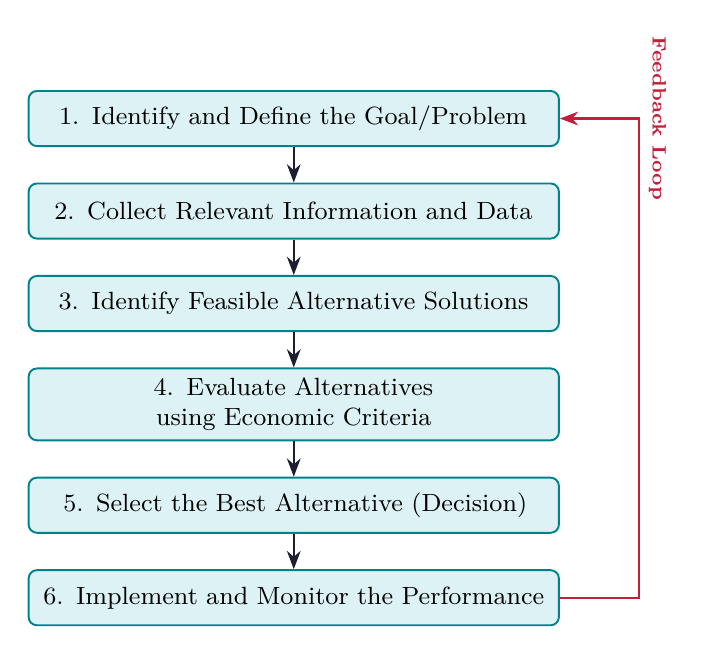
\begin{tikzpicture}[
  stepbox/.style={rectangle, draw=myteal, fill=hdrteal, text width=6.5cm,
    align=center, minimum height=0.7cm, font=\small, rounded corners=3pt, line width=0.7pt},
  flowarrow/.style={-Stealth, thick, color=mydark}
]
  \node[stepbox] (s1) {1. Identify and Define the Goal/Problem};
  \node[stepbox, below=0.45cm of s1] (s2) {2. Collect Relevant Information and Data};
  \node[stepbox, below=0.45cm of s2] (s3) {3. Identify Feasible Alternative Solutions};
  \node[stepbox, below=0.45cm of s3] (s4) {4. Evaluate Alternatives using Economic Criteria};
  \node[stepbox, below=0.45cm of s4] (s5) {5. Select the Best Alternative (Decision)};
  \node[stepbox, below=0.45cm of s5] (s6) {6. Implement and Monitor the Performance};

  \draw[flowarrow] (s1) -- (s2);
  \draw[flowarrow] (s2) -- (s3);
  \draw[flowarrow] (s3) -- (s4);
  \draw[flowarrow] (s4) -- (s5);
  \draw[flowarrow] (s5) -- (s6);

  % Feedback path
  \draw[flowarrow, color=myred] (s6.east) -- ++(1.0,0) |- (s1.east) 
    node[midway, above, rotate=-90, font=\scriptsize\bfseries\color{myred}] {Feedback Loop};
\end{tikzpicture}
\end{tcolorbox}

% ===============================================================================
\section{Engineering Costs and Estimation}
% ===============================================================================

To make sound economic decisions, engineers must understand the different classifications of costs.

\subsection{Fixed and Variable Costs}

\begin{tcolorbox}[defbox]
\textbf{Fixed Costs (FC):} Costs that remain constant in total, independent of the level of output or operational activity within a defined range. 
\par\vspace{3pt}
\textbf{Variable Costs (VC):} Costs that vary in direct proportion to the volume of output or activity level.
\end{tcolorbox}

\begin{tcolorbox}[formulabox, title={\textbf{Total Cost Equation}}]
The total cost ($TC$) for a production volume $q$ is expressed as:
\begin{equation}
  TC(q) = FC + VC(q) = FC + (v \times q)
\end{equation}
Where:
\begin{itemize}[leftmargin=1.5em, itemsep=1pt, topsep=2pt]
  \item[] $FC$ = Total Fixed Cost
  \item[] $VC(q)$ = Total Variable Cost for output $q$
  \item[] $v$ = Variable cost per unit of output
  \item[] $q$ = Quantity produced (output volume)
\end{itemize}
\end{tcolorbox}

\subsection{Marginal and Average Costs}

\begin{tcolorbox}[defbox]
\textbf{Marginal Cost (MC):} The incremental cost incurred by producing one additional unit of output.
\par\vspace{3pt}
\textbf{Average Cost (AC):} The total cost per unit of output produced.
\end{tcolorbox}

\begin{tcolorbox}[formulabox, title={\textbf{Average and Marginal Cost Formulas}}]
For a total cost function $TC(q)$:
\begin{align}
  AC(q) &= \frac{TC(q)}{q} = \frac{FC}{q} + v \\[6pt]
  MC(q) &= \frac{d(TC)}{dQ} \quad \text{(continuous)} \quad \text{or} \quad MC = \frac{\Delta TC}{\Delta q} \quad \text{(discrete)}
\end{align}
\end{tcolorbox}

\subsection{Sunk Costs and Opportunity Costs}

\begin{tcolorbox}[defbox]
\textbf{Sunk Cost:} A cost that has already been incurred in the past and cannot be recovered by any current or future action. Sunk costs are \textbf{irrelevant} for future-oriented decision-making.
\par\vspace{3pt}
\textbf{Opportunity Cost:} The benefit or return forgone (lost) by choosing a specific alternative over the next best alternative. It represents the value of resources in their best alternative use.
\end{tcolorbox}

\begin{tcolorbox}[exambox, title={\textbf{Exam Tip: The Sunk Cost Fallacy}}]
A common error in decision-making is trying to justify continuing an investment or project because "we have already spent so much money on it." In engineering economics, past expenditures are gone. Decisions must be based solely on future cash flows, incremental costs, and benefits.
\end{tcolorbox}

\subsection{Recurring and Nonrecurring Costs}
\begin{itemize}[leftmargin=*, itemsep=3pt]
  \item \textbf{Recurring Costs:} Expenses that occur repeatedly and predictably at regular intervals during the life cycle of an asset (e.g., annual maintenance, insurance, utility bills, raw material purchases).
  \item \textbf{Nonrecurring Costs:} One-time, non-repetitive expenses that occur at specific points, typically at the beginning or end of a project (e.g., initial research and development, land acquisition, equipment purchasing, installation, decommissioning costs).
\end{itemize}

\subsection{Incremental and Life-Cycle Costs}
\begin{itemize}[leftmargin=*, itemsep=3pt]
  \item \textbf{Incremental Cost:} The difference in total cost between two or more feasible alternatives. If Alternative A costs $\$12,000$ and Alternative B costs $\$15,000$, the incremental cost of choosing Alternative B over A is $\$3,000$.
  \item \textbf{Life-Cycle Cost (LCC):} The sum of all costs associated with a product, structure, system, or service over its entire life span. It covers all phases: acquisition, operation, maintenance, and disposal.
\end{itemize}

\subsection{Cash Costs vs. Book Costs}
It is critical to distinguish between transactions that involve real money and those that are purely accounting entries.\par\noindent
\begin{tabularx}{\linewidth}{|B{3.2cm}|Y|Y|}
\hline
\multicolumn{1}{|>{\centering\arraybackslash}m{3.2cm}|}{\textbf{Parameter}} &
\multicolumn{1}{>{\centering\arraybackslash}Y|}{\textbf{\color{myteal}Cash Cost}} &
\multicolumn{1}{>{\centering\arraybackslash}Y|}{\textbf{\color{myamber}Book Cost}} \\
\hline
\textbf{Definition} & Cost that involves an actual cash transaction or out-of-pocket payment. & Cost recorded in accounting books but does not involve a physical cash flow. \\
\hline
\textbf{Examples} & Purchase of raw materials, labor wages, utility bills, rent. & Depreciation of equipment, asset write-downs. \\
\hline
\textbf{Decision Role} & Directly used in economic analysis and cash flow calculations. & Mostly ignored in cash flow analysis (except for their impact on taxes). \\
\hline
\end{tabularx}

% ===============================================================================
\section{Cost Estimation Models}
% ===============================================================================

Cost estimation is the process of predicting the cost of a future engineering project or product.

\subsection{Types of Estimate}
Estimates vary in their detail, accuracy, and timing:
\begin{enumerate}[label=\textbf{\arabic*.}, leftmargin=*, itemsep=3pt, topsep=2pt]
  \item \textbf{Rough / Order-of-Magnitude Estimate:} Done during the initial conceptual phase. Accuracy is low ($\pm 30\%$). Uses historical data and simple scaling factors.
  \item \textbf{Semi-detailed / Budget Estimate:} Prepared during the preliminary design phase when major parameters are defined. Accuracy is moderate ($\pm 15\%$).
  \item \textbf{Detailed / Engineer's Estimate:} Prepared during the final design/bidding phase based on complete specifications and bills of materials. Accuracy is high ($\pm 5\%$).
\end{enumerate}

\subsection{Estimating Models}

\subsubsection{Per-Unit Model}
A simple model where the total cost is estimated by multiplying the number of units by a historical per-unit cost factor.
\begin{equation}
  C = U \times N
\end{equation}
Where $C$ is the total cost, $U$ is the cost per unit (e.g., cost per square foot of building space, cost per mile of highway), and $N$ is the number of units.

\subsubsection{Segmenting Model}
Estimates the total cost by dividing the project into individual components or segments, estimating the cost of each segment separately, and summing them.
\begin{equation}
  C = \sum_{i=1}^{m} C_i
\end{equation}
Where $C_i$ is the cost of segment $i$, and $m$ is the total number of segments. This is a bottom-up estimation technique.

\subsubsection{Cost Index Model}
Adjusts historical costs to present or future costs using cost indices that reflect inflation and changing economic conditions over time.

\begin{tcolorbox}[formulabox, title={\textbf{Cost Index Formula}}]
\begin{equation}
  C_t = C_0 \times \left( \frac{I_t}{I_0} \right)
\end{equation}
Where:
\begin{itemize}[leftmargin=1.5em, itemsep=1pt, topsep=2pt]
  \item[] $C_t$ = Estimated cost at time $t$ (present/future)
  \item[] $C_0$ = Historical cost at reference time $0$ (past)
  \item[] $I_t$ = Cost index value at time $t$
  \item[] $I_0$ = Cost index value at reference time $0$
\end{itemize}
\end{tcolorbox}

\subsubsection{Power-Sizing Model}
Used to estimate the cost of industrial equipment, plants, or facilities of different capacities. It accounts for economies of scale.

\begin{tcolorbox}[formulabox, title={\textbf{Power-Sizing Formula}}]
\begin{equation}
  C_A = C_B \times \left( \frac{S_A}{S_B} \right)^x
\end{equation}
Where:
\begin{itemize}[leftmargin=1.5em, itemsep=1pt, topsep=2pt]
  \item[] $C_A$ = Estimated cost of equipment/facility $A$
  \item[] $C_B$ = Historical cost of equipment/facility $B$
  \item[] $S_A$ = Size or capacity of equipment/facility $A$
  \item[] $S_B$ = Size or capacity of equipment/facility $B$
  \item[] $x$ = Sizing exponent (reflects economies of scale)
\end{itemize}
\par\vspace{4pt}
\textbf{The Six-Tenths Rule:} If the sizing exponent $x$ is unknown, a default value of $x = 0.6$ is often used (applicable to many chemical process reactors, tanks, and pumps).
\begin{itemize}[leftmargin=*, itemsep=2pt, topsep=2pt]
  \item[] $x < 1$: Economies of scale (cost increases slower than capacity).
  \item[] $x = 1$: Linear scaling (no scale advantage).
  \item[] $x > 1$: Diseconomies of scale (cost increases faster than capacity).
\end{itemize}
\end{tcolorbox}

\subsubsection{Improvement and Learning Curve Model}
Reflects the phenomenon where the direct labor hours required to perform a repetitive task decrease as the cumulative number of units produced increases.

\begin{tcolorbox}[formulabox, title={\textbf{Crawford's Learning Curve Model}}]
The time or cost to produce the $N$-th unit, $Z_N$, is given by:
\begin{equation}
  Z_N = K \times N^b
\end{equation}
Where:
\begin{itemize}[leftmargin=1.5em, itemsep=1pt, topsep=2pt]
  \item[] $Z_N$ = Time or cost required to produce the $N$-th unit
  \item[] $K$ = Time or cost required to produce the $1^{\text{st}}$ unit
  \item[] $N$ = Cumulative number of units produced
  \item[] $b$ = Learning exponent (index of learning)
\end{itemize}
\par\vspace{4pt}
The learning exponent $b$ is related to the learning rate $L$ (expressed as a decimal, e.g., $0.80$ for an $80\%$ curve) by:
\begin{equation}
  b = \frac{\log(L)}{\log(2)} = \frac{\ln(L)}{\ln(2)}
\end{equation}
Every time the cumulative production doubles (e.g., from 1 to 2, 2 to 4, 4 to 8), the time to produce that doubled unit is multiplied by the learning rate $L$:
\begin{equation}
  Z_{2N} = L \times Z_N
\end{equation}
\end{tcolorbox}

\subsection{Worked Examples}

\begin{tcolorbox}[examplebox, title={Example 1: Cost Index Model}]
\textbf{Problem:} In 2018, a company installed a heat exchanger at a cost of $\$85,000$. The plant cost index in 2018 was $560$. Estimate the cost of installing an identical heat exchanger in 2026, when the cost index is projected to be $840$.\\[4pt]
\textbf{Solution:}
Identify the given parameters:
\begin{itemize}[leftmargin=*, itemsep=1pt]
  \item[] Reference Cost $C_0 = \$85,000$
  \item[] Reference Index $I_0 = 560$
  \item[] Project Index $I_t = 840$
\end{itemize}
Using the Cost Index formula:
\begin{align*}
  C_{2026} &= C_0 \times \left( \frac{I_t}{I_0} \right) \\[4pt]
  C_{2026} &= 85,000 \times \left( \frac{840}{560} \right) \\[4pt]
  C_{2026} &= 85,000 \times 1.5 \\[4pt]
  C_{2026} &= \$127,500
\end{align*}
\textbf{Answer:} The estimated cost of the heat exchanger in 2026 is \textbf{\$127,500}.
\end{tcolorbox}

\begin{tcolorbox}[examplebox, title={Example 2: Power-Sizing Model}]
\textbf{Problem:} A water treatment plant with a capacity of $2.5$ million gallons per day (MGD) was constructed in 2020 for $\$3.2$ million. Estimate the cost of a similar plant with a capacity of $6.0$ MGD if the power-sizing exponent is $x = 0.68$.\\[4pt]
\textbf{Solution:}
Identify the given parameters:
\begin{itemize}[leftmargin=*, itemsep=1pt]
  \item[] Reference capacity $S_B = 2.5$ MGD, Reference cost $C_B = \$3,200,000$
  \item[] Target capacity $S_A = 6.0$ MGD
  \item[] Sizing exponent $x = 0.68$
\end{itemize}
Using the Power-Sizing formula:
\begin{align*}
  C_A &= C_B \times \left( \frac{S_A}{S_B} \right)^x \\[4pt]
  C_A &= 3,200,000 \times \left( \frac{6.0}{2.5} \right)^{0.68} \\[4pt]
  C_A &= 3,200,000 \times (2.4)^{0.68}
\end{align*}
Calculate the capacity ratio term:
\begin{align*}
  (2.4)^{0.68} &\approx 1.8155 \\[4pt]
  C_A &\approx 3,200,000 \times 1.8155 \\[4pt]
  C_A &\approx \$5,809,600
\end{align*}
\textbf{Answer:} The estimated cost of the 6.0 MGD plant is \textbf{\$5,809,600}.
\end{tcolorbox}

\begin{tcolorbox}[examplebox, title={Example 3: Learning Curve Model}]
\textbf{Problem:} The first prototype of a satellite communications receiver requires $80$ direct labor hours to assemble. The manufacturing line has an estimated learning rate of $85\%$.
\begin{enumerate}[label=\alph*., leftmargin=*, itemsep=2pt, topsep=2pt]
  \item Calculate the learning exponent $b$.
  \item Estimate the labor hours required to assemble the $8^{\text{th}}$ unit.
\end{enumerate}
\textbf{Solution:}
\textbf{(a) Calculate the learning exponent $b$:}
Using the formula $b = \frac{\log(L)}{\log(2)}$ with $L = 0.85$:
\begin{equation*}
  b = \frac{\log(0.85)}{\log(2)} \approx \frac{-0.07058}{0.30103} \approx -0.2345
\end{equation*}

\textbf{(b) Estimate labor hours for the $8^{\text{th}}$ unit ($N = 8$):}
\textit{Method 1: Direct Formula}
\begin{align*}
  Z_8 &= K \times 8^b \\
  Z_8 &= 80 \times 8^{-0.2345} \\
  Z_8 &\approx 80 \times 0.6141 \approx 49.13 \text{ hours}
\end{align*}
\textit{Method 2: Doubling Principle (Verification)}
Since $8$ is a double of $4$, which is a double of $2$, which is a double of $1$:
\begin{align*}
  Z_1 &= 80 \text{ hours} \\
  Z_2 &= 80 \times 0.85 = 68 \text{ hours} \\
  Z_4 &= 68 \times 0.85 = 57.8 \text{ hours} \\
  Z_8 &= 57.8 \times 0.85 = 49.13 \text{ hours}
\end{align*}
Both methods yield identical results.\\[4pt]
\textbf{Answer:} (a) The learning exponent $b$ is \textbf{-0.2345}. (b) The labor hours for the $8^{\text{th}}$ unit is \textbf{49.13 hours}.
\end{tcolorbox}

% ===============================================================================
% MANDATORY QUICK REVISION PAGE
% ===============================================================================
\newpage
\begin{center}
  {\large\bfseries\color{myred} Quick Revision --- Module I}\\[3pt]
  {\small\color{mydark} Introduction \& Cost Estimation $|$ HS-HU601}
\end{center}
\noindent{\color{myred}\rule{\linewidth}{1.2pt}}
\vspace{4pt}

\begin{tcolorbox}[formulabox, title={\textbf{Key Formulas at a Glance}}]
\renewcommand{\arraystretch}{1.3}
\begin{tabularx}{\linewidth}{B{3.8cm} X}
Total Cost              & $TC(q) = FC + VC = FC + (v \times q)$ \\[4pt]
Average Cost            & $AC(q) = \frac{TC(q)}{q} = \frac{FC}{q} + v$ \\[4pt]
Marginal Cost           & $MC(q) = \frac{d(TC)}{dq} \approx \frac{\Delta TC}{\Delta q}$ \\[4pt]
Cost Indexing           & $C_t = C_0 \times \left( \frac{I_t}{I_0} \right)$ \\[6pt]
Power-Sizing            & $C_A = C_B \times \left( \frac{S_A}{S_B} \right)^x$ \quad (six-tenths rule: $x = 0.6$) \\[6pt]
Learning Curve          & $Z_N = K \times N^b$ \\[4pt]
Learning Exponent       & $b = \frac{\log(L)}{\log(2)}$ \quad ($L$ = learning rate as a decimal)
\end{tabularx}
\end{tcolorbox}

\begin{tcolorbox}[defbox, title={\textbf{One-Line Definitions}}]
\begin{itemize}[leftmargin=*, itemsep=2pt, topsep=0pt]
  \item \textbf{Fixed Cost:} Expense that does not change with production output (e.g., rent, insurance).
  \item \textbf{Variable Cost:} Expense that increases or decreases proportionally with output volume (e.g., raw materials).
  \item \textbf{Sunk Cost:} Past expense that cannot be recovered; irrelevant for future decision-making.
  \item \textbf{Opportunity Cost:} The potential benefit lost by choosing one alternative over another.
  \item \textbf{Incremental Cost:} The change in total cost resulting from selecting one alternative over another.
  \item \textbf{Cash Cost:} Cost representing an out-of-pocket transaction involving actual cash flow.
  \item \textbf{Book Cost:} Recorded non-cash expense representing accounting transactions (e.g., depreciation).
  \item \textbf{Life-Cycle Cost:} The sum of all costs (acquisition, O\&M, disposal) over the lifespan of an asset.
\end{itemize}
\end{tcolorbox}

\begin{tcolorbox}[exambox, title={\textbf{Frequently Asked / Viva Questions}}]
\begin{enumerate}[topsep=0pt, label=\textbf{Q\arabic*.}, itemsep=5pt]
  \item \Q{What is the difference between physical and economic feasibility?}
    Physical feasibility ensures an engineering design is mechanically and structurally possible, while economic feasibility ensures it makes financial sense and yields a positive return.
  \item \Q{Why are sunk costs completely ignored in economic decision-making?}
    Sunk costs are historical expenditures that cannot be changed by any present or future choice. Only future incremental cash flows are affected by new decisions.
  \item \Q{Explain opportunity cost with a practical engineering example.}
    Opportunity cost is the profit forgone from an unselected alternative. For example, if a firm uses its warehouse for assembly rather than renting it out for $\$5,000$/month, the opportunity cost of assembly is $\$5,000$/month.
  \item \Q{What is the "six-tenths rule" in cost estimation?}
    The six-tenths rule is an empirical rule stating that the cost of a new facility/equipment of size $S_A$ is estimated as the cost of reference size $S_B$ multiplied by $(S_A/S_B)^{0.6}$.
  \item \Q{What is the difference between cash costs and book costs in engineering accounts?}
    Cash costs require an actual cash outflow (e.g., wages, raw materials). Book costs are accounting entries that do not involve cash flows (e.g., depreciation).
  \item \Q{How does the Crawford learning curve model function?}
    It states that the time to produce the $N$-th unit decreases exponentially according to $Z_N = K \times N^b$. Every time cumulative production doubles, unit labor time decreases by the learning rate.
  \item \Q{What does a power-sizing exponent $x < 1.0$ indicate?}
    It indicates economies of scale, meaning that doubling the capacity of the equipment will result in a cost increase of less than double ($2^x < 2$).
  \item \Q{Why is life-cycle cost (LCC) a better decision metric than initial acquisition cost?}
    An alternative with a lower purchase price may have high operating and maintenance costs. LCC accounts for all costs from acquisition to disposal, preventing long-term deficits.
  \item \Q{Distinguish between recurring and nonrecurring costs.}
    Recurring costs are periodic and repetitive (e.g., annual maintenance, monthly utility bills). Nonrecurring costs are one-time costs (e.g., land purchase, design costs).
  \item \Q{What are the typical accuracy ranges for the three major types of cost estimates?}
    Rough/Order-of-Magnitude estimate has an accuracy of $\pm 30\%$; Semi-detailed/Budget has $\pm 15\%$; and Detailed/Engineer's estimate has $\pm 5\%$.

  \item \Q{What is the sunk cost fallacy, and why is it dangerous in engineering projects?}
    It is the psychological tendency to continue investing in a failing project because of past non-recoverable expenditures, which leads to further losses.
  \item \Q{What are the components of the total cost equation, and how are average and marginal costs derived?}
    Total cost is $TC = FC + v \times q$. Average cost is derived by dividing total cost by quantity ($AC = FC/q + v$). Marginal cost is the derivative of total cost with respect to quantity ($MC = v$ for linear costs).
\end{enumerate}
\end{tcolorbox}

\begin{tcolorbox}[tikzbox, title={Comparison of Cost Estimating Models}]
\renewcommand{\arraystretch}{1.4}
\par\noindent
\begin{tabularx}{\linewidth}{|B{2.3cm}|Y|Y|Y|}
\hline
\textbf{Model Name} & \textbf{Core Formula} & \textbf{Data Needed} & \textbf{Primary Application} \\
\hline
\textbf{Per-Unit} & $C = U \times N$ & Historical unit rate $U$, quantity $N$ & Very early stage construction cost (e.g., cost per sq.\ ft.). \\
\hline
\textbf{Segmenting} & $C = \sum C_i$ & Detailed component cost breakdown & Detailed bottom-up estimates; bill of materials. \\
\hline
\textbf{Cost Index} & $C_t = C_0 \left( \frac{I_t}{I_0} \right)$ & Historical cost $C_0$, historical \& current indices & Adjusting past costs for inflation or price changes over time. \\
\hline
\textbf{Power-Sizing} & $C_A = C_B \left( \frac{S_A}{S_B} \right)^x$ & Size $S$, reference cost $C_B$, exponent $x$ & Estimating industrial equipment/plant capacity cost scaling. \\
\hline
\textbf{Learning Curve} & $Z_N = K \times N^b$ & First unit hours $K$, learning rate $L$ & Estimating labor costs for manufacturing assembly runs. \\
\hline
\end{tabularx}
\end{tcolorbox}


% -- Module 2 -----------------------------------------------------------------
\modulestart{2}{Cash Flow, Interest, and Equivalence}

\section{Cash Flow, Interest, and Equivalence}
% ===============================================================================

To evaluate engineering designs financially, we must track when money is spent and received.

\subsection{Cash Flow Diagrams}
A Cash Flow Diagram (CFD) is a graphical representation of cash flows plotted on a timeline.

\begin{tcolorbox}[defbox]
\textbf{Cash Inflow (Receipts):} Represented by vertical arrows pointing \textbf{upward} above the timeline (e.g., revenue, operating savings, salvage value).
\par\vspace{3pt}
\textbf{Cash Outflow (Disbursements):} Represented by vertical arrows pointing \textbf{downward} below the timeline (e.g., capital purchase, operating expenses, taxes).
\end{tcolorbox}

\begin{tcolorbox}[tikzbox, title={Typical Cash Flow Diagram for an Engineering Project}]
\centering
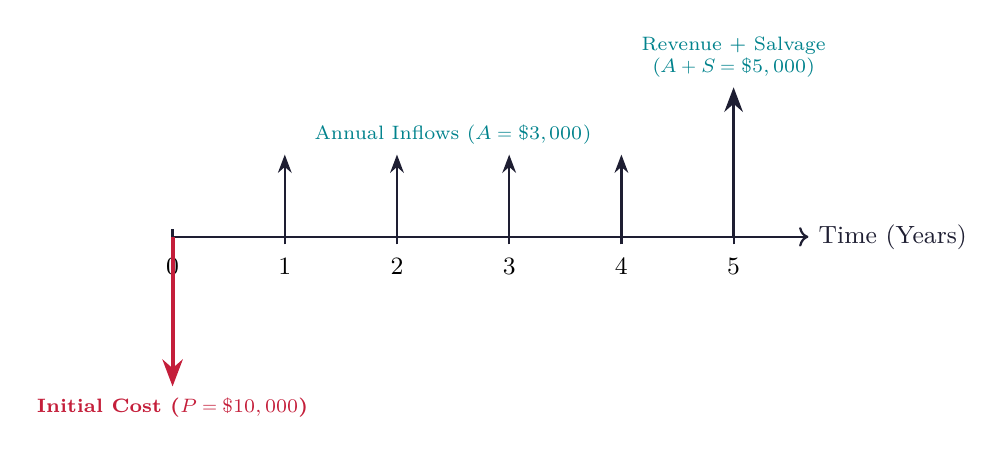
\begin{tikzpicture}[scale=0.95]
  % Timeline axis
  \draw[line, ->] (0,0) -- (8.5,0) node[right, font=\small] {Time (Years)};
  % Tick marks and labels
  \foreach \x/\lbl in {0/0, 1.5/1, 3.0/2, 4.5/3, 6.0/4, 7.5/5} {
    \draw[line] (\x, -0.1) -- (\x, 0.1);
    \node[below=4pt, font=\small] at (\x, 0) {\lbl};
  }
  
  % Outflow at t=0 (Initial Investment)
  \draw[redarrow, line width=1.5pt] (0,0) -- (0,-2.0) node[below, font=\scriptsize\bfseries\color{myred}] {Initial Cost ($P = \$10,000$)};
  
  % Annual Net Inflows at t=1..5
  \foreach \x/\t in {1.5/1, 3.0/2, 4.5/3, 6.0/4} {
    \draw[arrow] (\x,0) -- (\x, 1.1);
  }
  \node[above, font=\scriptsize\color{myteal}] at (3.75, 1.1) {Annual Inflows ($A = \$3,000$)};
  
  % Final Year inflow + Salvage Value at t=5
  \draw[arrow, line width=1.3pt] (7.5,0) -- (7.5, 2.0);
  \node[above, font=\scriptsize, align=center, color=myteal] at (7.5, 2.0) {Revenue + Salvage\\($A + S = \$5,000$)};
\end{tikzpicture}
\end{tcolorbox}

\subsection{Time Value of Money (TVM)}
The \textbf{Time Value of Money} states that a dollar received today is worth more than a dollar received in the future. This is due to three factors:
1.  \textbf{Opportunity Cost (Interest):} Capital can be invested to earn interest over time.
2.  \textbf{Inflation:} The purchasing power of money decreases over time.
3.  \textbf{Risk/Uncertainty:} Future receipts carry the risk of not being realized.

\subsection{Simple vs. Compound Interest}
\begin{itemize}[leftmargin=*, itemsep=6pt]
  \item \textbf{Simple Interest:} Calculated *only* on the original principal amount.
    \begin{equation}
      I = P \times i \times n
    \end{equation}
  \item \textbf{Compound Interest:} Interest is calculated on the principal *plus* any accumulated interest from previous periods.
    \begin{equation}
      F = P \times (1 + i)^n
    \end{equation}
\end{itemize}

\subsection{Nominal and Effective Interest Rates}
\begin{itemize}[leftmargin=*, itemsep=4pt]
  \item \textbf{Nominal Interest Rate ($r$):} The stated annual interest rate without considering compounding frequency within the year.
  \item \textbf{Effective Interest Rate ($i_a$):} The actual annual rate of interest paid or earned, accounting for compounding $m$ times per year.
\end{itemize}

\begin{tcolorbox}[formulabox, title={\textbf{Effective Interest Rate Formulas}}]
For a nominal rate $r$ compounded $m$ times per year:
\begin{equation}
  i_a = \left( 1 + \frac{r}{m} \right)^m - 1
\end{equation}
For continuous compounding ($m \to \infty$):
\begin{equation}
  i_a = e^r - 1
\end{equation}
\end{tcolorbox}

\subsection{Economic Equivalence}
Two cash flows (or series of cash flows) are \textbf{economically equivalent} at a given interest rate $i$ if they have the same financial value when discounted to the same point in time.

% ===============================================================================
\section{Time Value of Money Factors}
% ===============================================================================

To simplify calculations, standardized discount factors are used to convert cash flows between the Present ($P$), Future ($F$), and Uniform Series ($A$).


\subsection{TVM Factors Summary Table}
\par\noindent
{\renewcommand{\arraystretch}{1.9}%
\begin{tabularx}{\linewidth}{|B{3.2cm}|Y|Y|Y|}
\hline
\textbf{Find / Given} & \textbf{Factor Name} & \textbf{Standard Notation} & \textbf{Mathematical Formula} \\
\hline
Find $F$ given $P$ & Single Payment Compound Amount & $(F/P, i, n)$ & $(1+i)^n$ \\
\hline
Find $P$ given $F$ & Single Payment Present Worth & $(P/F, i, n)$ & $(1+i)^{-n}$ \\
\hline
Find $F$ given $A$ & Uniform Series Compound Amount & $(F/A, i, n)$ & $\displaystyle\frac{(1+i)^n - 1}{i}$ \\[6pt]
\hline
Find $A$ given $F$ & Sinking Fund & $(A/F, i, n)$ & $\displaystyle\frac{i}{(1+i)^n - 1}$ \\[6pt]
\hline
Find $A$ given $P$ & Capital Recovery & $(A/P, i, n)$ & $\displaystyle\frac{i(1+i)^n}{(1+i)^n - 1}$ \\[6pt]
\hline
Find $P$ given $A$ & Uniform Series Present Worth & $(P/A, i, n)$ & $\displaystyle\frac{(1+i)^n - 1}{i(1+i)^n}$ \\[6pt]
\hline
\end{tabularx}}


\subsection{Debt Repayment (Loan Amortization)}
Amortization is the process of paying off debt through a series of equal periodic payments.
Each payment $A$ consists of two parts:
1.  \textbf{Interest Portion ($I_t$):} Computed on the outstanding loan balance at the beginning of period $t$.
2.  \textbf{Principal Portion ($P_t$):} The remaining part of the payment that reduces the outstanding loan balance.

\begin{tcolorbox}[formulabox, title={\textbf{Loan Amortization Equations}}]
For a loan principal $P$ at interest rate $i$ repaid over $n$ periods:
\begin{align}
  \text{Equal annual payment: } A &= P \times (A/P, i, n) = P \times \frac{i(1+i)^n}{(1+i)^n - 1} \\[6pt]
  \text{Interest in period } t: I_t &= B_{t-1} \times i \quad \text{($B_{t-1}$ is outstanding balance)} \\[4pt]
  \text{Principal reduction in } t: P_t &= A - I_t \\[4pt]
  \text{Remaining balance after } t: B_t &= B_{t-1} - P_t
\end{align}
\end{tcolorbox}

% ===============================================================================
\section{Cash Flow and Rate of Return Analysis}
% ===============================================================================

Engineers use standard analysis methods to determine if a project is financially viable.

\subsection{Present Worth, Future Worth, and Annual Worth Analysis}
\begin{itemize}[leftmargin=*, itemsep=6pt]
  \item \textbf{Present Worth (PW) Analysis:} All cash inflows and outflows are discounted to the present ($t=0$) at the Minimum Attractive Rate of Return (MARR).
    \begin{equation}
      PW(i) = \sum_{t=0}^{n} CF_t \times (1 + i)^{-t}
    \end{equation}
    \textit{Decision Rule:} Accept the project if $PW(MARR) \ge 0$.
  \item \textbf{Future Worth (FW) Analysis:} Cash flows are compounded to a future point ($t=n$). Useful for determining net accumulation at the end of project life.
  \item \textbf{Annual Worth (AW) Analysis:} Cash flows are converted into an equivalent uniform series over the project life.
    \begin{equation}
      AW(i) = PW(i) \times (A/P, i, n)
    \end{equation}
    \textit{Decision Rule:} Accept the project if $AW(MARR) \ge 0$.
\end{itemize}

\subsection{Internal Rate of Return (IRR) Analysis}
The \textbf{Internal Rate of Return (IRR)} is the interest rate at which the Present Worth of all cash flows equals zero.

\begin{tcolorbox}[formulabox, title={\textbf{IRR Equation}}]
\begin{equation}
  PW(IRR) = \sum_{t=0}^{n} \frac{CF_t}{(1 + IRR)^t} = 0
\end{equation}
*Decision Rule:* Accept the project if $IRR \ge MARR$.
\par\vspace{3pt}
\textbf{Linear Interpolation formula:} If trial rates $i_1$ (giving $PW_1 > 0$) and $i_2$ (giving $PW_2 < 0$) are close:
\begin{equation}
  IRR \approx i_1 + \left( \frac{PW_1}{PW_1 - PW_2} \right) \times (i_2 - i_1)
\end{equation}
\end{tcolorbox}

\subsection{Benefit-Cost Ratio (BCR) Analysis}
Often used in public sector projects to assess whether the societal benefits justify the public expenditure.

\begin{tcolorbox}[formulabox, title={\textbf{Benefit-Cost Ratio Formula}}]
\begin{equation}
  BCR = \frac{PV(\text{Benefits})}{PV(\text{Costs})} = \frac{PW(\text{Cash Inflows})}{PW(\text{Cash Outflows})}
\end{equation}
*Decision Rule:* Accept the project if $BCR \ge 1.0$.
\end{tcolorbox}

\subsection{Sensitivity and Breakeven Analysis}
\begin{itemize}[leftmargin=*, itemsep=6pt]
  \item \textbf{Sensitivity Analysis:} Determines how financial metrics (like PW or IRR) change when key parameters (like initial cost, useful life, or annual revenue) deviate from their estimated values.
  \item \textbf{Breakeven Analysis:} Determines the value of a parameter (e.g., production capacity, price, number of years) at which two alternatives become economically equivalent. At the breakeven point:
    \begin{equation}
      PW_A(i) = PW_B(i) \quad \text{or} \quad AW_A(i) = AW_B(i)
    \end{equation}
\end{itemize}

% ===============================================================================
\section{Worked Examples}
% ===============================================================================

\begin{tcolorbox}[examplebox, title={Example 1: Nominal vs. Effective Interest}]
\textbf{Problem:} An engineering company deposits $\$10,000$ in a bank account that pays a nominal interest rate of $12\%$ per year. Calculate the effective annual interest rate and the total balance after $5$ years under:
\begin{enumerate}[label=\alph*., leftmargin=*, itemsep=2pt, topsep=2pt]
  \item Quarterly compounding ($m = 4$).
  \item Continuous compounding.
\end{enumerate}
\textbf{Solution:}\\[4pt]
\textbf{(a) Quarterly Compounding ($m = 4$):}
\begin{align*}
  i_a &= \left( 1 + \frac{r}{m} \right)^m - 1 = \left( 1 + \frac{0.12}{4} \right)^4 - 1 = (1.03)^4 - 1 \\
  i_a &\approx 1.1255 - 1 = 12.55\%
\end{align*}
Future Balance after $5$ years ($n = 5 \times 4 = 20$ quarters, interest rate per quarter $= 3\%$):
\begin{align*}
  F &= P(1 + i)^{n_{quarters}} = 10,000 \times (1.03)^{20} \\
  F &\approx 10,000 \times 1.8061 = \$18,061
\end{align*}

\textbf{(b) Continuous Compounding:}
\begin{align*}
  i_a &= e^r - 1 = e^{0.12} - 1 \approx 1.1275 - 1 = 12.75\%
\end{align*}
Future Balance after $5$ years:
\begin{align*}
  F &= P \times e^{r \times t} = 10,000 \times e^{0.12 \times 5} = 10,000 \times e^{0.60} \\
  F &\approx 10,000 \times 1.8221 = \$18,221
\end{align*}
\textbf{Answer:} (a) Effective rate $= \mathbf{12.55\%}$, Balance $= \mathbf{\$18,061}$. (b) Effective rate $= \mathbf{12.75\%}$, Balance $= \mathbf{\$18,221}$.
\tcbset{breakable}
\end{tcolorbox}

\begin{tcolorbox}[examplebox, title={Example 2: Loan Amortization Schedule}]
\textbf{Problem:} A manufacturing startup borrows $\$50,000$ to buy CNC tooling. The loan is to be repaid in $5$ equal annual installments at a compound interest rate of $8\%$ per year. Calculate the annual payment and find the interest and principal components for Year 1.\\[4pt]
\textbf{Solution:}
Identify given parameters: Principal $P = \$50,000$, Rate $i = 0.08$, Periods $n = 5$.
Calculate the equal annual payment $A$ using Capital Recovery factor $(A/P, 8\%, 5)$:
\begin{align*}
  A &= P \times \frac{i(1+i)^n}{(1+i)^n - 1} = 50,000 \times \frac{0.08(1.08)^5}{(1.08)^5 - 1} \\[4pt]
  A &= 50,000 \times \frac{0.08 \times 1.4693}{1.4693 - 1} = 50,000 \times 0.25046 = \$12,523
\end{align*}
Calculate components for \textbf{Year 1}:
\begin{align*}
  \text{Initial balance } B_0 &= \$50,000 \\
  \text{Interest portion } I_1 &= B_0 \times i = 50,000 \times 0.08 = \$4,000 \\
  \text{Principal portion } P_1 &= A - I_1 = 12,523 - 4,000 = \$8,523 \\
  \text{Ending balance } B_1 &= B_0 - P_1 = 50,000 - 8,523 = \$41,477
\end{align*}
\textbf{Answer:} The equal annual payment is \textbf{\$12,523}. In Year 1, the Interest paid is \textbf{\$4,000} and the Principal reduction is \textbf{\$8,523}.
\end{tcolorbox}

\begin{tcolorbox}[examplebox, title={Example 3: Internal Rate of Return (IRR)}]
\textbf{Problem:} An energy efficiency project requires an initial outlay of $\$25,000$ and generates net annual savings of $\$6,500$ for $5$ years. Find the IRR of this project using linear interpolation.\\[4pt]
\textbf{Solution:}
The cash flows are: $CF_0 = -\$25,000$, $CF_{1..5} = +\$6,500$ (Annuity).
We need to find $i$ such that $PW(i) = 0$:
\begin{align*}
  PW(i) = -25,000 + 6,500 \times (P/A, i, 5) = 0 \quad \Rightarrow \quad (P/A, i, 5) = \frac{25,000}{6,500} \approx 3.8462
\end{align*}
Let's try trial interest rates:
1.  \textbf{Try $i_1 = 9\%$:}
    \begin{align*}
      (P/A, 9\%, 5) &= \frac{(1.09)^5 - 1}{0.09(1.09)^5} \approx 3.8897 \\
      PW(9\%) &= -25,000 + 6,500 \times 3.8897 = -25,000 + 25,283 = +\$283 \quad (\text{above zero})
    \end{align*}
2.  \textbf{Try $i_2 = 10\%$:}
    \begin{align*}
      (P/A, 10\%, 5) &= \frac{(1.10)^5 - 1}{0.10(1.10)^5} \approx 3.7908 \\
      PW(10\%) &= -25,000 + 6,500 \times 3.7908 = -25,000 + 24,640 = -\$360 \quad (\text{below zero})
    \end{align*}
Using linear interpolation between $i_1 = 9\%$ and $i_2 = 10\%$:
\begin{align*}
  IRR &\approx i_1 + \left( \frac{PW(i_1)}{PW(i_1) - PW(i_2)} \right) \times (i_2 - i_1) \\
  IRR &\approx 0.09 + \left( \frac{283}{283 - (-360)} \right) \times (0.10 - 0.09) \\
  IRR &\approx 0.09 + \left( \frac{283}{643} \right) \times 0.01 \approx 0.09 + 0.44 \times 0.01 = 9.44\%
\end{align*}
\textbf{Answer:} The estimated Internal Rate of Return (IRR) is \textbf{9.44\%}.
\end{tcolorbox}

% ===============================================================================
% MANDATORY QUICK REVISION PAGE
% ===============================================================================
\newpage
\begin{center}
  {\large\bfseries\color{myred} Quick Revision --- Module II}\\[3pt]
  {\small\color{mydark} Interest \& Rate of Return $|$ HS-HU601}
\end{center}
\noindent{\color{myred}\rule{\linewidth}{1.2pt}}
\vspace{4pt}

\begin{tcolorbox}[formulabox, title={\textbf{Key Formulas at a Glance}}]
\renewcommand{\arraystretch}{1.3}
\begin{tabularx}{\linewidth}{B{3.8cm} X}
Effective Interest      & $i_a = (1 + r/m)^m - 1$ \quad (Continuous compounding: $i_a = e^r - 1$) \\[4pt]
Single payment PW       & $P = F \times (1 + i)^{-n}$ \\[4pt]
Capital Recovery        & $A = P \times \displaystyle\frac{i(1+i)^n}{(1+i)^n - 1}$ \\[6pt]
Uniform series PW       & $P = A \times \displaystyle\frac{(1+i)^n - 1}{i(1+i)^n}$ \\[6pt]
IRR Interpolation       & $IRR \approx i_1 + \displaystyle\frac{PW_1}{PW_1 - PW_2} \times (i_2 - i_1)$ \\[6pt]
Benefit-Cost Ratio      & $BCR = \displaystyle\frac{PV(\text{Benefits})}{PV(\text{Costs})} = \frac{PW(\text{Inflows})}{PW(\text{Outflows})}$
\end{tabularx}
\end{tcolorbox}

\begin{tcolorbox}[defbox, title={\textbf{One-Line Definitions}}]
\begin{itemize}[leftmargin=*, itemsep=2pt, topsep=0pt]
  \item \textbf{Cash Flow Diagram:} Graphic representation of cash receipts (up) and disbursements (down) over time.
  \item \textbf{Nominal Interest Rate:} Stated annual interest rate without considering sub-year compounding.
  \item \textbf{Effective Interest Rate:} The actual annual rate of interest paid, accounting for compounding periods.
  \item \textbf{Amortization:} Paying off debt in equal installments, consisting of both principal and interest.
  \item \textbf{Present Worth (PW):} The value of future net cash flows discounted to the present at the MARR.
  \item \textbf{Annual Worth (AW):} Equivalent annual uniform series of a project's cash flows over its lifetime.
  \item \textbf{Internal Rate of Return:} The discount rate that makes the Present Worth of all cash flows equal zero.
  \item \textbf{Benefit-Cost Ratio:} Ratio of present worth of benefits to present worth of costs (must be $\ge 1.0$).
  \item \textbf{Breakeven Point:} The value of a parameter at which two investment alternatives are economically equivalent.
\end{itemize}
\end{tcolorbox}

\begin{tcolorbox}[exambox, title={\textbf{Frequently Asked / Viva Questions}}]
\begin{enumerate}[topsep=0pt, label=\textbf{Q\arabic*.}, itemsep=5pt]
  \item \Q{What is economic equivalence?}
    Two different cash flow streams are equivalent at a specific interest rate if they have the same financial value when discounted to the same point in time.
  \item \Q{What is the difference between nominal and effective interest rates?}
    Nominal rate is the annual rate ignoring sub-year compounding frequency. Effective rate represents the actual annual interest earned, accounting for compounding within the year.
  \item \Q{How does the principal and interest portion change in loan amortization?}
    Over time, as the outstanding principal balance decreases, the interest portion of the fixed payment decreases, while the principal repayment portion increases.
  \item \Q{Define the Sinking Fund factor $(A/F, i, n)$.}
    It determines the uniform annual payment ($A$) needed to accumulate a specific future sum ($F$) after $n$ years at interest rate $i$.
  \item \Q{State the decision criteria for Present Worth and Annual Worth analysis.}
    A project is economically viable if its Present Worth ($PW$) or Annual Worth ($AW$), evaluated at the MARR, is greater than or equal to zero ($\ge 0$).
  \item \Q{What is the Minimum Attractive Rate of Return (MARR)?}
    The minimum interest rate a company requires on its capital investments before accepting a project, based on its cost of capital and risk.
  \item \Q{How is the Internal Rate of Return (IRR) calculated?}
    By setting the $PW(i) = 0$ and solving for $i$. In practice, it is solved by finding two rates where $PW$ changes sign and interpolating linearly between them.
  \item \Q{Why is continuous compounding relevant in engineering economics?}
    It represents the limit as compounding frequency approaches infinity. It is used in advanced financial modeling and for automated, continuous transactions.
  \item \Q{Explain the Benefit-Cost Ratio decision rule.}
    If $BCR \ge 1.0$, the discounted benefits exceed the discounted costs, meaning the project is acceptable. If $BCR < 1.0$, the project is rejected.
  \item \Q{What is the purpose of sensitivity analysis in engineering designs?}
    It assesses how variations or uncertainty in estimated parameters (e.g., initial cost, salvage value, inflation) affect the project's profitability.

  \item \Q{Define the Capital Recovery factor $(A/P, i, n)$ and explain its economic meaning.}
    It represents the equivalent annual cost of owning an asset, combining both the initial purchase depreciation and the interest cost on the invested capital.
  \item \Q{What occurs at the breakeven point between two engineering alternatives?}
    The two alternatives become economically equivalent, meaning their present worths or annual worths are identical. Choosing either alternative yields the same economic result.
\end{enumerate}
\tcbset{breakable}
\end{tcolorbox}

\begin{tcolorbox}[tikzbox, title={Comparison of TVM Factors and Operations}]
\renewcommand{\arraystretch}{1.45}
\par\noindent
\begin{tabularx}{\linewidth}{|B{2.3cm}|Y|Y|Y|}
\hline
\textbf{Factor Symbol} & \textbf{Name} & \textbf{Core Formula} & \textbf{Typical Application} \\
\hline
\textbf{$(F/P, i, n)$} & Compound Amount & $(1+i)^n$ & Finding the future value of a single deposit. \\
\hline
\textbf{$(P/F, i, n)$} & Present Worth & $(1+i)^{-n}$ & Discounting a single future payment back to present. \\
\hline
\textbf{$(F/A, i, n)$} & Uniform Compound & $\displaystyle\frac{(1+i)^n - 1}{i}$ & Accumulating a pension fund through yearly deposits. \\
\hline
\textbf{$(A/P, i, n)$} & Capital Recovery & $\displaystyle\frac{i(1+i)^n}{(1+i)^n - 1}$ & Determining equal annual mortgage or loan payments. \\
\hline
\textbf{$(P/A, i, n)$} & Uniform Present & $\displaystyle\frac{(1+i)^n - 1}{i(1+i)^n}$ & Evaluating the present worth of uniform annual savings. \\
\hline
\end{tabularx}
\end{tcolorbox}


% -- Module 3 -----------------------------------------------------------------
\modulestart{3}{Inflation and Price Change}

\section{Inflation and Price Change}
% ===============================================================================

Financial plans made in a stable environment can fail when prices rise over time.

\subsection{Inflation Concepts}
\begin{tcolorbox}[defbox]
\textbf{Inflation:} A general and progressive increase in the prices of goods and services over time, resulting in a decline in the purchasing power of money.
\par\vspace{3pt}
\textbf{Consumer Price Index (CPI):} A measure that examines the weighted average of prices of a basket of consumer goods and services. It is used to estimate price changes.
\end{tcolorbox}

\subsection{Interest Rates under Inflation (Fisher's Equation)}
Inflation separates the interest rate earned into a \textbf{nominal (market) rate} and a \textbf{real rate}.
\begin{itemize}[leftmargin=*, itemsep=4pt]
  \item \textbf{Nominal Interest Rate ($i$):} The actual interest rate paid or earned in the market.
  \item \textbf{Real Interest Rate ($i'$):} The interest rate adjusted to represent the real increase in purchasing power.
  \item \textbf{Inflation Rate ($f$):} The rate at which the price index increases.
\end{itemize}

\begin{tcolorbox}[formulabox, title={\textbf{Fisher's Equation}}]
The relationship between nominal interest, real interest, and inflation is:
\begin{equation}
  1 + i = (1 + i') \times (1 + f)
\end{equation}
Expanding this gives:
\begin{equation}
  i = i' + f + (i' \times f)
\end{equation}
To find the real interest rate:
\begin{equation}
  i' = \frac{i - f}{1 + f}
\end{equation}
\end{tcolorbox}

\subsection{Differential Inflation Rates}
Different components of a project (e.g., fuel, labor, equipment) may inflate at different rates. If a specific cost inflates at rate $f_j$, its future cash flow in year $t$ is:
\begin{equation}
  CF_t = CF_0 \times (1 + f_j)^t
\end{equation}
This is then discounted back to present using the market interest rate $i$.

% ===============================================================================
\section{Present Worth Analysis \& Mutual Exclusivity}
% ===============================================================================

When comparing competing engineering projects, specific conventions must be followed.

\subsection{Project Comparison Viewpoints}
1.  \textbf{Economic Studies Viewpoint:} Assesses the project based on total investment capital, ignoring how the project is financed.
2.  \textbf{Borrowed Money Viewpoint:} Includes the cash flows of borrowing (receipt of loan principal) and debt repayment (interest and principal payments).

\subsection{Effect of Income Taxes}
Corporate income taxes reduce net cash inflows.
\begin{itemize}[leftmargin=*, itemsep=4pt]
  \item $\text{Taxable Income} = \text{Revenues} - \text{Operating Expenses} - \text{Depreciation}$
  \item $\text{Income Tax} = \text{Taxable Income} \times \text{Corporate Tax Rate } (t)$
  \item \textbf{Tax Depreciation Shield:} Depreciation is a non-cash expense that reduces taxable income, shielding the company from taxes. The annual tax savings equal:
    \begin{equation}
      \text{Tax Shield} = t \times d_t \quad \text{($d_t$ is the depreciation in year $t$)}
    \end{equation}
\end{itemize}

\subsection{Comparing Projects with Unequal Lives}
We cannot compare the Present Worth of two alternatives directly if they have different useful lives because the service periods differ.
\begin{itemize}[leftmargin=*, itemsep=6pt]
  \item \textbf{Least Common Multiple (LCM) Method:} Compare projects over a study period equal to the LCM of their lives. It assumes that each alternative will be replaced at the end of its life with an identical asset at the same cost.
  \item \textbf{Co-termination (Study Period) Method:} A fixed study period is selected (e.g., 5 years). Any alternative with a shorter life is replaced, and any alternative with a longer life is assigned a salvage value at the end of the study period.
\end{itemize}

% ===============================================================================
\section{Uncertainty in Future Events}
% ===============================================================================

Engineering estimates of future costs and revenues are rarely certain.

\subsection{Expected Value}
When future cash flows are uncertain but can be assigned probabilities:
\begin{tcolorbox}[formulabox, title={\textbf{Expected Value Formula}}]
The expected value ($E[X]$) of a random cash flow variable $X$ is:
\begin{equation}
  E[X] = \sum_{j=1}^{M} x_j \times P(x_j)
\end{equation}
Where $x_j$ is the cash flow under outcome $j$, $P(x_j)$ is its probability, and $M$ is the number of outcomes.
\end{tcolorbox}

\subsection{Economic Decision Trees}
A decision tree is a graphical tool used to analyze decisions under risk.
\begin{itemize}[leftmargin=*, itemsep=4pt]
  \item \textbf{Decision Nodes (Squares):} Points where the decision-maker must select an alternative.
  \item \textbf{Chance Nodes (Circles):} Points where outcomes are determined by probability.
  \item \textbf{Branches:} Connect nodes; chance branches show probabilities and outcomes.
\end{itemize}

\begin{tcolorbox}[tikzbox, title={Economic Decision Tree for Plant Expansion}]
\centering
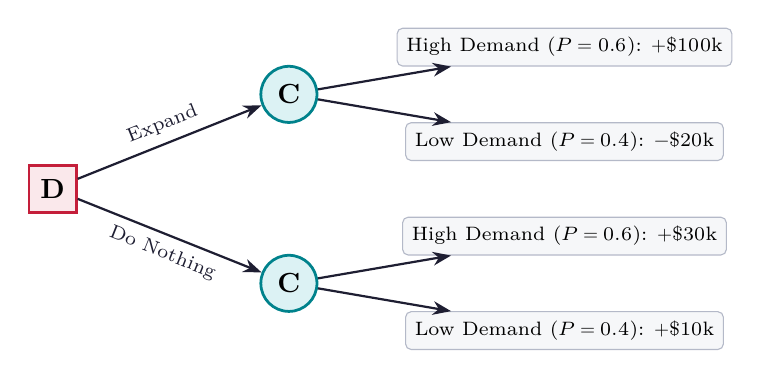
\begin{tikzpicture}[
  dnode/.style={rectangle, draw=myred, fill=hdrred, minimum size=0.6cm, line width=1.0pt},
  cnode/.style={circle, draw=myteal, fill=hdrteal, minimum size=0.6cm, line width=1.0pt},
  leaf/.style={rectangle, draw=mgframe, fill=mygray, font=\scriptsize, rounded corners=2pt},
  arrow/.style={-Stealth, thick, color=mydark}
]
  % Root Decision Node
  \node[dnode] (D1) at (0,0) {\textbf{D}};
  
  % Chance Nodes
  \node[cnode] (C1) at (3, 1.2) {\textbf{C}};
  \node[cnode] (C2) at (3, -1.2) {\textbf{C}};
  
  % Leaf Nodes
  \node[leaf] (L1) at (6.5, 1.8) {High Demand ($P=0.6$): $+\$100\text{k}$};
  \node[leaf] (L2) at (6.5, 0.6) {Low Demand ($P=0.4$): $-\$20\text{k}$};
  \node[leaf] (L3) at (6.5, -0.6) {High Demand ($P=0.6$): $+\$30\text{k}$};
  \node[leaf] (L4) at (6.5, -1.8) {Low Demand ($P=0.4$): $+\$10\text{k}$};
  
  % Connect D1 to C1 and C2
  \draw[arrow] (D1) -- node[above, sloped, font=\scriptsize] {Expand} (C1);
  \draw[arrow] (D1) -- node[below, sloped, font=\scriptsize] {Do Nothing} (C2);
  
  % Connect C1 to L1, L2
  \draw[arrow] (C1) -- (L1);
  \draw[arrow] (C1) -- (L2);
  
  % Connect C2 to L3, L4
  \draw[arrow] (C2) -- (L3);
  \draw[arrow] (C2) -- (L4);
\end{tikzpicture}
\end{tcolorbox}

% ===============================================================================
\section{Worked Examples}
% ===============================================================================

\begin{tcolorbox}[examplebox, title={Example 1: Fisher's Equation}]
\textbf{Problem:} An electronics engineer wants to earn a real rate of return of $6\%$ per year on an investment. If inflation is projected to run at an average rate of $4\%$ per year over the next few years, what nominal market interest rate must the investment yield?\\[4pt]
\textbf{Solution:}
Identify given parameters: Real interest rate $i' = 0.06$, Inflation rate $f = 0.04$.
Using Fisher's Equation:
\begin{align*}
  i &= i' + f + (i' \times f) \\
  i &= 0.06 + 0.04 + (0.06 \times 0.04) \\
  i &= 0.10 + 0.0024 \\
  i &= 0.1024 = 10.24\%
\end{align*}
\textbf{Alternative check using $(1+i)$:}
\begin{align*}
  1 + i &= (1 + i')(1 + f) = (1.06) \times (1.04) = 1.1024 \quad \Rightarrow \quad i = 10.24\%
\end{align*}
\textbf{Answer:} The investment must yield a nominal market interest rate of \textbf{10.24\%}.
\end{tcolorbox}

\begin{tcolorbox}[examplebox, title={Example 2: Mutually Exclusive Projects with Unequal Lives}]
\textbf{Problem:} Compare two manufacturing machines at an interest rate of $10\%$ using the Present Worth method.
\begin{itemize}[leftmargin=*, itemsep=3pt, topsep=2pt]
  \item \textbf{Machine A:} Initial cost $= \$10,000$, useful life $= 2$ years, annual operating cost $= \$2,000$.
  \item \textbf{Machine B:} Initial cost $= \$15,000$, useful life $= 3$ years, annual operating cost $= \$1,500$.
\end{itemize}
\vspace{4pt}
\textbf{Solution:}
The lives are unequal ($2$ and $3$ years). The study period must be the Least Common Multiple:
\begin{equation*}
  \text{Study Period} = \text{LCM}(2, 3) = 6 \text{ years}
\end{equation*}
\begin{itemize}[leftmargin=*, itemsep=8pt]
  \item \textbf{Machine A (re-purchased at end of Year 2 and Year 4):} \\
    Cash outflows occur at $t=0$ ($\$10\text{k}$), $t=2$ ($\$10\text{k}$), $t=4$ ($\$10\text{k}$), and annual costs of $\$2\text{k}$ for Years $1..6$.
    \begin{align*}
      PW_A(10\%) &= -10,000 - 10,000 \times (P/F, 10\%, 2) - 10,000 \times (P/F, 10\%, 4) \\
                 & \quad - 2,000 \times (P/A, 10\%, 6) \\
      PW_A(10\%) &= -10,000 - 10,000(0.8264) - 10,000(0.6830) - 2,000(4.3553) \\
      PW_A(10\%) &= -10,000 - 8,264 - 6,830 - 8,711 = -\$33,805
    \end{align*}
  \item \textbf{Machine B (re-purchased at end of Year 3):} \\
    Cash outflows occur at $t=0$ ($\$15\text{k}$), $t=3$ ($\$15\text{k}$), and annual costs of $\$1.5\text{k}$ for Years $1..6$.
    \begin{align*}
      PW_B(10\%) &= -15,000 - 15,000 \times (P/F, 10\%, 3) - 1,500 \times (P/A, 10\%, 6) \\
      PW_B(10\%) &= -15,000 - 15,000(0.7513) - 1,500(4.3553) \\
      PW_B(10\%) &= -15,000 - 11,270 - 6,533 = -\$32,803
    \end{align*}
\end{itemize}
Comparing the Present Worths over 6 years:
\begin{align*}
  PW_B (-\$32,803) &> PW_A (-\$33,805) \quad (\text{Machine B has lower net present cost})
\end{align*}
\textbf{Answer:} \textbf{Machine B} is selected since it minimizes the net present cost over the 6-year study period.
\end{tcolorbox}

\begin{tcolorbox}[examplebox, title={Example 3: Decision Tree Rollback}]
\textbf{Problem:} Roll back the plant expansion decision tree shown in Section 3.2. Find the expected value for each alternative and determine the optimal decision.\\[4pt]
\textbf{Solution:}
Calculate the Expected Value (EV) for each decision branch:
1.  \textbf{Branch 1: Expand}
    The outcomes are High Demand ($+\$100\text{k}$ at $P=0.6$) and Low Demand ($-\$20\text{k}$ at $P=0.4$).
    \begin{align*}
      EV(\text{Expand}) &= 100,000 \times 0.6 + (-20,000) \times 0.4 \\
                        &= 60,000 - 8,000 = \$52,000
    \end{align*}
2.  \textbf{Branch 2: Do Nothing}
    The outcomes are High Demand ($+\$30\text{k}$ at $P=0.6$) and Low Demand ($+\$10\text{k}$ at $P=0.4$).
    \begin{align*}
      EV(\text{Do Nothing}) &= 30,000 \times 0.6 + 10,000 \times 0.4 \\
                            &= 18,000 + 4,000 = \$22,000
    \end{align*}
Compare expected values at the root decision node:
\begin{align*}
  EV(\text{Expand}) = \$52,000 &> EV(\text{Do Nothing}) = \$22,000
\end{align*}
The optimal choice is to select the path with the highest expected value.
\par\vspace{3pt}
\textbf{Answer:} The optimal decision is to \textbf{Expand}, with an expected value of \textbf{\$52,000}.
\end{tcolorbox}

% ===============================================================================
% MANDATORY QUICK REVISION PAGE
% ===============================================================================
\newpage
\begin{center}
  {\large\bfseries\color{myred} Quick Revision --- Module III}\\[3pt]
  {\small\color{mydark} Inflation, Present Worth \& Uncertainty $|$ HS-HU601}
\end{center}
\noindent{\color{myred}\rule{\linewidth}{1.2pt}}
\vspace{4pt}

\begin{tcolorbox}[formulabox, title={\textbf{Key Formulas at a Glance}}]
\renewcommand{\arraystretch}{1.3}
\begin{tabularx}{\linewidth}{B{3.8cm} X}
Fisher's Equation       & $i = i' + f + i'f$ \\[4pt]
Real Interest Rate      & $i' = \displaystyle\frac{i - f}{1 + f}$ \\[6pt]
Tax Depreciation Shield & $\text{Tax Savings} = t \times d_t$ \quad ($t$ = tax rate, $d_t$ = depreciation) \\[4pt]
Expected Value          & $E[X] = \displaystyle\sum x_j P(x_j)$ \\[6pt]
LCM Study Period        & Study Period = Least Common Multiple of individual project lives
\end{tabularx}
\end{tcolorbox}

\begin{tcolorbox}[defbox, title={\textbf{One-Line Definitions}}]
\begin{itemize}[leftmargin=*, itemsep=2pt, topsep=0pt]
  \item \textbf{CPI:} An index measuring inflation by tracking average price changes of consumer goods.
  \item \textbf{Real Interest Rate:} The rate of return adjusted to reflect actual increases in purchasing power.
  \item \textbf{Tax Shield:} The reduction in income tax liability resulting from tax-deductible depreciation.
  \item \textbf{LCM Method:} Project comparison method over a study period matching the least common multiple of their lives.
  \item \textbf{Co-termination:} Comparing alternatives over a fixed study period, assigning salvage value to remaining assets.
  \item \textbf{Expected Value:} Weighted average of all possible numerical outcomes, using probabilities as weights.
  \item \textbf{Decision Tree:} Graphical model displaying sequential decisions, probabilities, and financial outcomes.
  \item \textbf{Monte Carlo Simulation:} Computational algorithm that uses repeated random sampling to model uncertainty.
\end{itemize}
\end{tcolorbox}

\begin{tcolorbox}[exambox, title={\textbf{Frequently Asked / Viva Questions}}]
\begin{enumerate}[topsep=0pt, label=\textbf{Q\arabic*.}, itemsep=5pt]
  \item \Q{How does inflation affect the value of cash flows over time?}
    Inflation reduces the purchasing power of money, meaning future cash flows are worth less in real terms than nominal terms.
  \item \Q{State Fisher's Equation and define its variables.}
    $i = i' + f + i'f$, where $i$ is the nominal market interest rate, $i'$ is the real interest rate, and $f$ is the inflation rate.
  \item \Q{What is the difference between the economic studies and borrowed money viewpoints?}
    Economic studies viewpoint evaluates a project based on total capital requirements, ignoring financing. Borrowed money viewpoint includes the loan receipts and debt payments.
  \item \Q{How does depreciation act as a tax shield?}
    Depreciation is a non-cash expense that is subtracted from revenue to calculate taxable income. By lowering taxable income, it reduces corporate tax liability.
  \item \Q{Why can we not compare PW of unequal-life alternatives directly?}
    Because the alternatives do not provide service over the same timeframe. Comparing them directly over different lives violates the equal-service comparison rule.
  \item \Q{Describe the assumption behind the Least Common Multiple (LCM) method.}
    It assumes that each alternative can be replaced at the end of its life with an identical asset having the same initial cost and operating costs.
  \item \Q{Explain the co-termination method for comparing unequal-life projects.}
    A specific study period is chosen. Shorter-lived alternatives are replaced, and longer-lived alternatives are terminated early, assigning them a salvage value.
  \item \Q{What is the difference between decision nodes and chance nodes in a decision tree?}
    Decision nodes (squares) represent points where the engineer has control over choices. Chance nodes (circles) represent points where outcomes occur based on probability.
  \item \Q{How do we roll back (solve) a decision tree?}
    We work from right to left (backwards). At each chance node, we calculate the expected value. At each decision node, we select the branch with the highest value.
  \item \Q{What does a high risk-premium imply for a project's MARR?}
    High-risk projects require a higher risk-premium, which increases the Minimum Attractive Rate of Return (MARR) used to discount its cash flows.

  \item \Q{What is the purpose of Monte Carlo simulation in risk analysis?}
    It allows the engineer to model parameters as probability distributions rather than single-point estimates, generating a distribution of possible PW outcomes.
  \item \Q{What are Real Options in engineering project management?}
    The managerial flexibility to adapt decisions in response to market changes, such as the option to expand, contract, defer, or abandon a project.
\end{enumerate}
\end{tcolorbox}

\begin{tcolorbox}[tikzbox, title={Comparison of Project Selection Methods under Equivalence}]
\renewcommand{\arraystretch}{1.45}
\par\noindent
\begin{tabularx}{\linewidth}{|B{2.3cm}|Y|Y|Y|}
\hline
\textbf{Method} & \textbf{Core Metric} & \textbf{Study Period Rule} & \textbf{Primary Application} \\
\hline
\textbf{Present Worth (PW)} & Net present value at $t=0$ & Must be equal (use LCM for unequal lives) & Comparing mutually exclusive projects with defined lives. \\
\hline
\textbf{Annual Worth (AW)} & Equivalent uniform annual series & Equal to useful life (does not require LCM) & Comparing alternatives with unequal service lives easily. \\
\hline
\textbf{IRR} & Discount rate where $PW = 0$ & Compare IRR to MARR; requires incremental analysis & Evaluating single projects or ranking capital budgets. \\
\hline
\textbf{BCR} & Ratio of discounted benefits to costs & Equal study period required & Public sector projects and government infrastructure. \\
\hline
\end{tabularx}
\end{tcolorbox}


% -- Module 4 -----------------------------------------------------------------
\modulestart{4}{Depreciation Calculations}

\section{Depreciation Calculations}
% ===============================================================================

Assets lose value over time, which affects taxes and company value.

\subsection{Depreciation Concepts}
\begin{tcolorbox}[defbox]
\textbf{Depreciation:} The systematic allocation of the cost of a tangible asset over its useful life to represent wear, tear, physical deterioration, or obsolescence.
\par\vspace{3pt}
\textbf{Book Value ($BV_t$):} The remaining value of an asset recorded in accounting books after subtracting accumulated depreciation from the initial cost.
\end{tcolorbox}

\subsection{Straight-Line (SL) Depreciation}
The simplest method; allocates an equal amount of depreciation to each year of the asset's life.
\begin{tcolorbox}[formulabox, title={\textbf{Straight-Line Formulas}}]
For initial cost $C$, salvage value $S$, and useful life $n$:
\begin{align}
  \text{Annual depreciation: } d_t &= \frac{C - S}{n} \\[4pt]
  \text{Book value in year } t: BV_t &= C - (t \times d_t)
\end{align}
\end{tcolorbox}

\subsection{Declining Balance (DB) \& Double Declining Balance (DDB)}
An accelerated method where depreciation is calculated as a fixed percentage of the remaining book value.
\begin{tcolorbox}[formulabox, title={\textbf{Declining Balance Formulas}}]
The depreciation rate $\alpha$ is given by:
\begin{equation}
  \alpha = \frac{\text{Factor}}{n} \quad \text{(For Double Declining Balance DDB, Factor = 2)}
\end{equation}
Annual depreciation, book value, and accumulated depreciation calculations:
\begin{align}
  \text{Depreciation in year } t: d_t &= \alpha \times BV_{t-1} \\[4pt]
  \text{Book value in year } t: BV_t &= C \times (1 - \alpha)^t
\end{align}
*Note: An asset cannot be depreciated below its salvage value. Once $BV_t$ reaches $S$, depreciation stops.*
\end{tcolorbox}

% ===============================================================================
\section{Replacement Analysis}
% ===============================================================================

Replacement analysis determines when an existing asset should be replaced by a new one.

\subsection{Economic Service Life (ESL)}
The \textbf{Economic Service Life (ESL)} is the asset life $k^*$ that minimizes the total equivalent annual cost. It is the optimum point that balances capital costs and rising operating costs.

\begin{tcolorbox}[formulabox, title={\textbf{Total Annual Cost Equation}}]
The Total Annual Cost ($ATC$) of owning an asset for $k$ years at interest rate $i$ is:
\begin{equation}
  ATC(k) = CR(k) + AEC_{O\&M}(k)
\end{equation}
Where:
\begin{align}
  \text{Capital Recovery cost: } CR(k) &= [C - S_k(P/F, i, k)] \times (A/P, i, k) \\[4pt]
  \text{Equivalent Annual O\&M: } AEC_{O\&M}(k) &= \left[ \sum_{t=1}^{k} O\&M_t \times (P/F, i, t) \right] \times (A/P, i, k)
\end{align}
\end{tcolorbox}

\subsection{Defender vs. Challenger Comparison}
\begin{itemize}[leftmargin=*, itemsep=4pt]
  \item \textbf{Defender (D):} The existing asset currently in use.
  \item \textbf{Challenger (C):} The best available replacement candidate.
\end{itemize}

\begin{tcolorbox}[tikzbox, title={Replacement Decision Process Flowchart}]
\centering
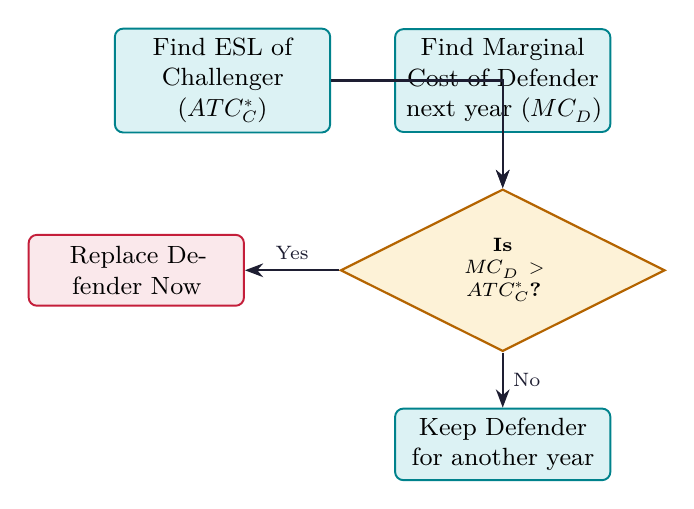
\begin{tikzpicture}[
  node distance=0.4cm and 0.8cm,
  sblock/.style={rectangle, draw=myteal, fill=hdrteal, text width=2.5cm,
    align=center, minimum height=0.9cm, font=\small, rounded corners=3pt, line width=0.7pt},
  rblock/.style={rectangle, draw=myred, fill=hdrred, text width=2.5cm,
    align=center, minimum height=0.9cm, font=\small, rounded corners=3pt, line width=0.7pt},
  decision/.style={diamond, draw=myamber, fill=hdramber, aspect=2, text width=1.8cm,
    align=center, font=\scriptsize\bfseries, line width=0.8pt}
]
  \node[sblock] (n1) {Find ESL of Challenger ($ATC_C^*$)};
  \node[sblock, right=0.8cm of n1] (n2) {Find Marginal Cost of Defender next year ($MC_D$)};
  \node[decision, below=0.7cm of n2] (d1) {Is\\$MC_D > ATC_C^*$?};
  \node[rblock, left=1.2cm of d1] (rep) {Replace Defender Now};
  \node[sblock, below=0.7cm of d1] (keep) {Keep Defender for another year};
  
  \draw[arrow] (n1) -| (d1.north);
  \draw[arrow] (n2) -- (d1.north);
  \draw[arrow] (d1) -- node[above, font=\scriptsize] {Yes} (rep);
  \draw[arrow] (d1) -- node[right, font=\scriptsize] {No} (keep);
\end{tikzpicture}
\end{tcolorbox}

\textbf{Marginal Cost of Defender next year:}
\begin{equation}
  MC_D(t+1) = (MV_t - MV_{t+1}) + (MV_t \times i) + O\&M_{t+1}
\end{equation}
Where $MV_t$ is current market value, $MV_{t+1}$ is market value next year, and $O\&M_{t+1}$ is operating cost next year.

% ===============================================================================
\section{Basic Accounting for Engineers}
% ===============================================================================

Engineers must understand financial statements and cost allocation to make business decisions.

\subsection{Financial Statements}
1.  \textbf{Balance Sheet:} Represents a snapshot of the firm's financial position at a specific point in time. It satisfies the fundamental accounting equation:
    \begin{equation}
      \text{Assets} = \text{Liabilities} + \text{Owner's Equity}
    \end{equation}
2.  \textbf{Income Statement:} Summarizes revenues and expenses over a period of time (e.g., quarter or year) to calculate net income:
    \begin{equation}
      \text{Net Income} = \text{Revenues} - \text{Expenses}
    \end{equation}

\subsection{Financial Ratios}
\begin{itemize}[leftmargin=*, itemsep=6pt]
  \item \textbf{Liquidity (Current Ratio):} $\text{Current Ratio} = \displaystyle\frac{\text{Current Assets}}{\text{Current Liabilities}}$
  \item \textbf{Profitability (Return on Equity):} $ROE = \displaystyle\frac{\text{Net Income}}{\text{Owner's Equity}}$
  \item \textbf{Leverage (Debt-to-Equity):} $\text{Debt-to-Equity} = \displaystyle\frac{\text{Total Liabilities}}{\text{Owner's Equity}}$
\end{itemize}

\subsection{Cost Accounting and Allocation}
\begin{itemize}[leftmargin=*, itemsep=4pt]
  \item \textbf{Direct Costs:} Costs directly traceable to a product or service (e.g., direct materials, assembly labor).
  \item \textbf{Indirect Costs (Overhead):} Costs that cannot be easily traced to a specific product (e.g., building rent, supervisor salaries, factory electricity).
  \item \textbf{Indirect Cost Allocation:} Distributing overhead costs to products using allocation bases like direct labor hours, machine hours, or direct material costs.
\end{itemize}

% ===============================================================================
\section{Worked Examples}
% ===============================================================================

\begin{tcolorbox}[examplebox, title={Example 1: Double Declining Balance (DDB)}]
\textbf{Problem:} A test instrument costs $\$80,000$, has a useful life of $5$ years, and a salvage value of $\$10,000$. Calculate the depreciation amount and book value for Year 1 and Year 2 using the DDB method.\\[4pt]
\textbf{Solution:}
Identify parameters: Cost $C = \$80,000$, Life $n = 5$, Salvage value $S = \$10,000$.
Calculate DDB rate $\alpha$:
\begin{equation*}
  \alpha = \frac{2}{n} = \frac{2}{5} = 0.40 \quad (40\% \text{ per year})
\end{equation*}
\begin{itemize}[leftmargin=*, itemsep=8pt]
  \item \textbf{Year 1:}
    \begin{align*}
      \text{Depreciation: } d_1 &= \alpha \times BV_0 = 0.40 \times 80,000 = \$32,000 \\
      \text{Book Value: } BV_1 &= C - d_1 = 80,000 - 32,000 = \$48,000
    \end{align*}
  \item \textbf{Year 2:}
    \begin{align*}
      \text{Depreciation: } d_2 &= \alpha \times BV_1 = 0.40 \times 48,000 = \$19,200 \\
      \text{Book Value: } BV_2 &= BV_1 - d_2 = 48,000 - 19,200 = \$28,800
    \end{align*}
\end{itemize}
Since $BV_2 = \$28,800 > S = \$10,000$, we do not need to adjust for the salvage value floor yet.\\[4pt]
\textbf{Answer:} Year 1: Depreciation $= \mathbf{\$32,000}$, Book Value $= \mathbf{\$48,000}$. Year 2: Depreciation $= \mathbf{\$19,200}$, Book Value $= \mathbf{\$28,800}$.
\end{tcolorbox}

\begin{tcolorbox}[examplebox, title={Example 2: Replacement Analysis}]
\textbf{Problem:} An existing compressor (defender) has a current market value of $\$5,000$. If kept for another year, its market value will fall to $\$3,500$ and operating costs will be $\$6,500$. A new compressor (challenger) has a minimum annual cost of $\$8,000$. At an interest rate of $10\%$, should the company replace the compressor now?\\[4pt]
\textbf{Solution:}
Calculate the Marginal Cost of the defender ($MC_D$) for next year:
\begin{itemize}[leftmargin=*, itemsep=2pt, topsep=2pt]
  \item Current market value $MV_t = \$5,000$, Market value next year $MV_{t+1} = \$3,500$.
  \item Interest rate $i = 0.10$.
  \item Operating and Maintenance cost $O\&M_{t+1} = \$6,500$.
\end{itemize}
\begin{align*}
  MC_D &= (MV_t - MV_{t+1}) + (MV_t \times i) + O\&M_{t+1} \\
  MC_D &= (5,000 - 3,500) + (5,000 \times 0.10) + 6,500 \\
  MC_D &= 1,500 + 500 + 6,500 = \$8,500
\end{align*}
Compare $MC_D$ next year with the minimum annual cost of the challenger ($ATC_C^* = \$8,000$):
\begin{align*}
  MC_D (\$8,500) &> ATC_C^* (\$8,000) \quad (\text{Keeping defender is more expensive})
\end{align*}
Since the marginal cost of keeping the defender exceeds the annual cost of the challenger, the defender should be replaced.\\[4pt]
\textbf{Answer:} \textbf{Replace now}, as keeping the defender for another year costs $\$8,500$ compared to the challenger's annual cost of $\$8,000$.
\end{tcolorbox}

\begin{tcolorbox}[examplebox, title={Example 3: Indirect Cost Allocation}]
\textbf{Problem:} A workshop incurs factory overhead costs of $\$12,000$. It produces two products: Product A (requires $400$ direct labor hours) and Product B (requires $800$ direct labor hours). Allocate the overhead cost to both products using direct labor hours as the allocation base.\\[4pt]
\textbf{Solution:}
Identify parameters: Total Overhead $= \$12,000$, Total Labor Hours $= 400 + 800 = 1,200$ hours.
Calculate the overhead allocation rate:
\begin{align*}
  \text{Allocation Rate} &= \frac{\text{Total Overhead}}{\text{Total Labor Hours}} = \frac{12,000}{1,200} = \$10 \text{ per labor hour}
\end{align*}
Allocate overhead to each product:
\begin{itemize}[leftmargin=*, itemsep=8pt]
  \item \textbf{Product A:}
    \begin{align*}
      \text{Allocated Overhead} &= 400 \text{ hours} \times \$10/\text{hour} = \$4,000
    \end{align*}
  \item \textbf{Product B:}
    \begin{align*}
      \text{Allocated Overhead} &= 800 \text{ hours} \times \$10/\text{hour} = \$8,000
    \end{align*}
\end{itemize}
Verification: $\$4,000 + \$8,000 = \$12,000$ (total overhead allocated).\\[4pt]
\textbf{Answer:} \textbf{Product A} is allocated \textbf{\$4,000} and \textbf{Product B} is allocated \textbf{\$8,000}.
\end{tcolorbox}

% ===============================================================================
% MANDATORY QUICK REVISION PAGE
% ===============================================================================
\newpage
\begin{center}
  {\large\bfseries\color{myred} Quick Revision --- Module IV}\\[3pt]
  {\small\color{mydark} Depreciation, Replacement \& Accounting $|$ HS-HU601}
\end{center}
\noindent{\color{myred}\rule{\linewidth}{1.2pt}}
\vspace{4pt}

\begin{tcolorbox}[formulabox, title={\textbf{Key Formulas at a Glance}}]
\renewcommand{\arraystretch}{1.3}
\begin{tabularx}{\linewidth}{B{3.8cm} X}
Straight-Line Dep.      & $d_t = \displaystyle\frac{C - S}{n}$ \quad ($BV_t = C - t \times d_t$) \\[6pt]
Declining Balance Dep.  & $d_t = \alpha \times BV_{t-1}$ \quad ($BV_t = C \times (1 - \alpha)^t$) \\[4pt]
DDB Rate                & $\alpha = \displaystyle\frac{2}{n}$ \\[6pt]
Capital Recovery        & $CR(k) = [C - S_k(P/F, i, k)] \times (A/P, i, k)$ \\[4pt]
Defender Marginal Cost  & $MC_D(t+1) = (MV_t - MV_{t+1}) + (MV_t \times i) + O\&M_{t+1}$ \\[4pt]
Accounting Equation     & $\text{Assets} = \text{Liabilities} + \text{Owner's Equity}$ \\[4pt]
Current Ratio           & $\text{Current Ratio} = \displaystyle\frac{\text{Current Assets}}{\text{Current Liabilities}}$
\end{tabularx}
\end{tcolorbox}

\begin{tcolorbox}[defbox, title={\textbf{One-Line Definitions}}]
\begin{itemize}[leftmargin=*, itemsep=2pt, topsep=0pt]
  \item \textbf{Depreciation:} Allocation of an asset's cost over its life to account for wear and tear.
  \item \textbf{Book Value:} Cost of an asset minus accumulated depreciation.
  \item \textbf{Economic Service Life:} The asset life that minimizes total equivalent annual cost.
  \item \textbf{Defender:} An existing asset currently owned and operating.
  \item \textbf{Challenger:} The best replacement candidate available.
  \item \textbf{Balance Sheet:} Statement showing assets, liabilities, and equity at a specific point in time.
  \item \textbf{Income Statement:} Statement showing revenues, expenses, and net profit over a period.
  \item \textbf{Direct Cost:} Expense directly traceable to a product (e.g., labor, raw materials).
  \item \textbf{Indirect Cost:} Expense that cannot be easily traced to a product (e.g., rent, utilities).
\end{itemize}
\end{tcolorbox}

\begin{tcolorbox}[exambox, title={\textbf{Frequently Asked / Viva Questions}}]
\begin{enumerate}[topsep=0pt, label=\textbf{Q\arabic*.}, itemsep=5pt]
  \item \Q{What is the difference between physical deterioration and obsolescence?}
    Physical deterioration is wear and tear due to usage or environmental factors. Obsolescence is the loss of value due to technological progress (newer, better alternatives).
  \item \Q{Explain the Straight-Line depreciation method.}
    It allocates an equal amount of depreciation to each year of the asset's useful life: $d_t = (C-S)/n$.
  \item \Q{What is the salvage value floor rule in Declining Balance methods?}
    An asset cannot be depreciated below its salvage value. Once the book value ($BV_t$) drops to the salvage value ($S$), depreciation must stop.
  \item \Q{Define the Economic Service Life (ESL) of an asset.}
    The period of ownership that minimizes the sum of equivalent annual capital recovery costs and annual operating and maintenance costs.
  \item \Q{What costs are included in the Capital Recovery cost ($CR$) of an asset?}
    The annualized cost of depreciation (loss in asset value) and the interest cost on the capital invested in the asset.
  \item \Q{How is the defender's marginal cost for next year calculated?}
    By adding the projected loss in market value, the interest on its current market value, and the operating and maintenance costs for next year.
  \item \Q{State the decision rule in Defender vs. Challenger replacement analysis.}
    If the marginal cost of keeping the defender for one more year is greater than the minimum annual cost of the challenger, replace the defender immediately.
  \item \Q{State the fundamental accounting equation.}
    $\text{Assets} = \text{Liabilities} + \text{Owner's Equity}$. It forms the basis of the Balance Sheet.
  \item \Q{What is the difference between direct and indirect costs in manufacturing?}
    Direct costs can be traced directly to a product (e.g., material). Indirect costs cannot be traced directly and must be allocated (e.g., factory rent).
  \item \Q{What is the Current Ratio, and what does it measure?}
    Current Assets divided by Current Liabilities. It measures a firm's liquidity (ability to pay off short-term debts).

  \item \Q{Explain the concept of overhead cost allocation.}
    The process of distributing indirect costs (like supervisor salaries or utilities) to different products using an allocation base like direct labor hours.
  \item \Q{What is the Double Declining Balance (DDB) depreciation rate?}
    It is twice the straight-line rate: $\alpha = 2/n$. It represents accelerated depreciation in the early years of asset ownership.
\end{enumerate}
\end{tcolorbox}

\begin{tcolorbox}[tikzbox, title={Comparison of Depreciation Methods}]
\renewcommand{\arraystretch}{1.45}
\par\noindent
\begin{tabularx}{\linewidth}{|B{2.3cm}|Y|Y|Y|}
\hline
\textbf{Method} & \textbf{Depreciation Pattern} & \textbf{Calculation Base} & \textbf{Primary Use} \\
\hline
\textbf{Straight-Line} & Constant annual depreciation & $(C-S)$ is constant & Standard accounting; simple financial reporting. \\
\hline
\textbf{Declining Balance} & Accelerated; higher in early years & Remaining book value ($BV_{t-1}$) & Assets that lose value quickly (vehicles, computers). \\
\hline
\textbf{Double Declining} & Maximum acceleration rate ($2/n$) & Remaining book value ($BV_{t-1}$) & Tax reporting (maximizes early tax shields). \\
\hline
\textbf{Sinking Fund} & Increases over time & $(C-S)$ with interest & Special asset funds; rarely used in modern tax accounting. \\
\hline
\end{tabularx}
\end{tcolorbox}


\end{document}
